\documentclass[10pt,a4paper]{article}
\usepackage[a4paper,margin=19mm]{geometry}
\usepackage[T1]{fontenc}
\usepackage[utf8]{inputenc}
\usepackage{lmodern}
\usepackage{microtype}
\usepackage{booktabs}
\usepackage{tabularx}
\usepackage{array}
\usepackage{enumitem}
\usepackage{caption}
\usepackage{float}
\usepackage{tikz}
\usetikzlibrary{positioning,arrows.meta}
\usepackage[hidelinks]{hyperref}

\setlist{nosep,topsep=2pt,leftmargin=*}
\captionsetup{font=small,skip=3pt}
\setlength{\parskip}{3pt}
\setlength{\parindent}{0pt}
\newcolumntype{Y}{>{\raggedright\arraybackslash}X}
\newcolumntype{R}{>{\raggedleft\arraybackslash}p{1.05cm}}
\newcommand{\code}[1]{\texttt{#1}}
\renewcommand{\arraystretch}{1.05}

\title{\vspace{-8mm}NoticeCheck: Checking the Procedure of GST Tax Demands\\with a Small Language Model}
\author{Team Bleed Tokens\\[1pt]
\small Neill Rawani (2025202027) \quad Tanisha Upadhayay (2025201088) \quad Aryan (2025201017) \quad Rajarshi Chatterjee (2025814004)\\[1pt]
\small LMA Group Project 2026 \quad 15 November 2026\\[1pt]
\small Code and data: \url{https://github.com/neill-nil/gst-scn-compliance-audit}}
\date{\vspace{-5mm}}

\begin{document}
\maketitle

%==========================================================
\begin{abstract}
\noindent When an Indian GST officer demands unpaid tax, the law requires a fixed procedure: a proper notice, a chance to reply, a personal hearing and a reasoned order passed on time. High Courts regularly cancel demands that skip a step, yet most small businesses cannot tell whether their own case was handled correctly. NoticeCheck reads the record of a demand proceeding and checks each required step. For 13 kinds of procedural defect it answers \emph{defect}, \emph{no defect}, \emph{can't tell} or \emph{contested}, cites the section of the law, quotes the record as evidence, and says when a lawyer should take over. It runs on a free 8-billion-parameter model (Qwen3-8B) with planning, tools, statute lookup and a verifier around it, plus a LoRA-tuned copy of the same model that extracts the facts from a document. We built a test set of 125 real High Court cases labelled by the court's own findings and checked by our team (Cohen's $\kappa = 0.73$). When a defect only counts if the cited section is also right, NoticeCheck beats the same model used directly by 23--32 F1 points (95\% intervals above zero) and raises a third as many flags on points nobody argued. It roughly matches a large commercial model (Gemini) at finding defects and cites the law more accurately. Fine-tuning raises fact-extraction F1 from 0.52 to 0.80. Recall stays low for every system, mainly because court judgments often omit the facts a check needs.
\end{abstract}

%==========================================================
\section{Introduction}

\textbf{The problem.} Under India's Goods and Services Tax (GST), a tax officer who believes a business paid too little tax starts a \emph{demand proceeding} under Section 73 of the CGST Act, 2017 \cite{cgst} (no fraud alleged) or Section 74 (fraud or suppression alleged, with a longer time limit). The law fixes the steps: a show cause notice (Form DRC-01) stating the grounds, time for the business to reply, a personal hearing before any adverse decision (s.75(4)), an order that gives reasons and stays within the notice (s.75(6), s.75(7)), proper service of each document (s.169), and an order within the time limit (s.73(10), s.74(10)). Notices are issued in very large numbers, often uploaded to an online portal that small firms rarely check. When a step is skipped, High Courts set the demand aside, and thousands of such writ petitions have been filed in the last two years.

\textbf{Who needs help, and how.} Most GST-registered businesses are sole proprietors without a tax team. A shop owner who receives a demand order cannot easily tell whether a hearing was actually offered, whether the reply was considered, or whether the order came too late. Missing a real defect means paying a demand that a court would have cancelled; being told wrongly that a notice is invalid can make someone ignore a real demand and lose the chance to appeal. Three kinds of user benefit from a careful checker:
\begin{itemize}
\item \textbf{Small taxpayers}, who get a plain list of what may have gone wrong, with the law and the evidence for each point, and a clear signal when to see a professional.
\item \textbf{Tax practitioners and lawyers}, who can screen many cases quickly instead of checking the same list by hand each time.
\item \textbf{Tax officers}, who can check their own proceeding before passing an order, since a procedural defect usually sends the case back for a fresh hearing.
\end{itemize}

\textbf{What NoticeCheck does.} The user provides the record of the proceeding: the notice, the reply, hearing dates and the order. NoticeCheck returns a report covering 13 defect types. Each entry has a verdict (\emph{defect}, \emph{no defect}, \emph{can't tell}, or \emph{contested} where courts disagree), the section behind it, quotes from the record, and the facts it would need when it cannot decide. It also decides whether to hand the case to a professional, for example when a reply deadline is days away. It checks procedure only and never says whether tax is owed.

\textbf{Why this is hard for a language model.} A general chatbot asked about a notice tends to answer confidently, cite the wrong section, and flag problems that are not there. The checks also need exact date arithmetic (time limits depend on annual-return due dates and on extension notifications whose validity is still disputed), and some points of law are unsettled. We therefore wrap a small model in a fixed structure: it plans which tools to call, simple checks run as code, judgment calls go to the model one question at a time with the statute text attached, and a verifier rejects any defect that does not quote the record.

\textbf{Research questions.}
\textbf{RQ1:} Does this structured checking find procedural defects better than the same small model given the record directly? Our proposal fixed the test in advance: defect-level F1 where both the defect type and the cited section must match the answer key, judged as failed if the gain is under 10 points or its 95\% interval includes zero, if the false-alarm rate is higher than the baseline's, or if the system does not beat a rule checklist on defects that need reasoning.
\textbf{RQ2:} Can the same 8B model, fine-tuned with LoRA, extract the facts of a proceeding as well as a large prompted model?

%==========================================================
\section{Literature review}

\textbf{Language models in law.} Benchmarks such as LexGLUE \cite{lexglue} and LegalBench \cite{legalbench} show that large models handle many legal reading tasks but struggle with rule application and multi-step reasoning. Statutory reasoning in tax law has its own benchmark (SARA) \cite{sara}, where models misapply simple statutes \cite{blairstanek}, while newer models improve when the relevant statute text is supplied \cite{nay}. Studies of legal hallucination report that general models invent case law and misstate holdings \cite{dahl}, and that even commercial legal research tools built on retrieval still produce unsupported answers \cite{magesh}. Indian legal NLP has mostly targeted judgment prediction \cite{ildc} and the structure of judgments \cite{rhetorical}, not checking whether an administrative procedure was followed.

\textbf{Retrieval, tools and verification.} Retrieval-augmented generation grounds answers in a document collection \cite{rag}, and citation-focused work measures whether cited text actually supports an answer \cite{alce}. Models can call external tools for facts and arithmetic \cite{toolformer} and interleave reasoning with actions \cite{react}. Step-by-step prompting improves multi-step reasoning \cite{cot}. Our pipeline borrows the idea of reading in stages with an explicit ``not present'' answer and a sufficiency check from IntrAgent \cite{intragent}.

\textbf{Small models and fine-tuning.} LoRA \cite{lora} and QLoRA \cite{qlora} adapt a model by training small added matrices, which makes fine-tuning an 8B model possible on a single free GPU. We use Qwen3-8B \cite{qwen3} for both checking and extraction.

\textbf{Gap.} We found no benchmark or system for checking the procedure of tax demands against a statute, scored against what courts actually decided. NoticeCheck and its test set address that gap.

%==========================================================
\section{Dataset}

\textbf{Why court judgments.} Real show cause notices are confidential. High Court judgments are public, describe the whole proceeding (notice, reply, hearing, order), and then rule on each complaint. One judgment therefore gives both the facts and the right answer. We use the official eCourts judgments published on the AWS Open Data registry under CC-BY-4.0 \cite{awsdata}; other legal websites were used only to find case names.

\textbf{From 20,000 judgments to a test set.}
\begin{enumerate}
\item \textbf{Screening.} We screened 20,087 GST judgments from 24 High Courts (2024--2026) with keyword rules: about 4,900 concerned a s.73/74 demand, and 429 contained a real ruling on a procedural complaint. Most of the rest were short orders sending cases back by consent, which rule on nothing.
\item \textbf{Cleaning.} PDFs were turned into numbered paragraphs. Cleaning only deletes boilerplate lines (page stamps, signature notices); it never rewrites text, so every quote can be checked against the original.
\item \textbf{Drafting.} Gemini 3.5 Flash Lite drafted a structured record for 425 judgments: the facts (section invoked, financial years, notice and order dates, hearing, service, events, what the notice, reply and order said) and the court's finding on each complaint, with a verbatim quote and paragraph number for every value.
\item \textbf{Human review.} The four of us corrected every draft against the judgment in a review tool we built, which checks each quote word for word. A value without a verified quote is not used.
\end{enumerate}

\textbf{Labels.} For each complaint the answer key records whether the court found a defect, rejected the complaint, or did not decide it (for example, a remand ``for one more opportunity''). Undecided complaints are never scored. Points of law where courts disagree are marked \emph{contested}.

\begin{table}[H]
\centering\small
\begin{tabularx}{\textwidth}{l r Y}
\toprule
Set & Cases & Use \\
\midrule
Test & 125 & all main results; 208 complaints: 104 defects found, 38 rejected, 66 not decided \\
Held-out court (Karnataka) & 12 & a court never seen while building the system; 6 defects found \\
Development & 49 & tuning only (14 fully reviewed) \\
Fresh check & 20 & picked after the system was frozen; outputs checked by hand (Section~\ref{sec:fresh}) \\
Fine-tuning data & 196 + 21 & Gemini drafts of other judgments, for training and validating the extractor \\
\bottomrule
\end{tabularx}
\caption{Data splits. Courts in the gold set: Madras 52, Delhi 27, Allahabad 18, Karnataka 12, Bombay 10, others 18.}
\end{table}

\textbf{Label quality.} Thirty-five cases were labelled twice independently. Agreement on the court's findings is Cohen's $\kappa = 0.73$ \cite{cohen} over 58 complaints (0.75 on the pairs labelled without AI help); disagreements were settled by one team member and logged.

\textbf{What the system sees.} The system receives only the facts of the proceeding. The court's reasoning, findings and outcome are removed, and a check confirms none survive. We test two views: the \emph{full record}, and \emph{notice only}, which contains just what was known on the day the notice was issued.

%==========================================================
\section{Methodology}

\begin{figure}[H]
\centering
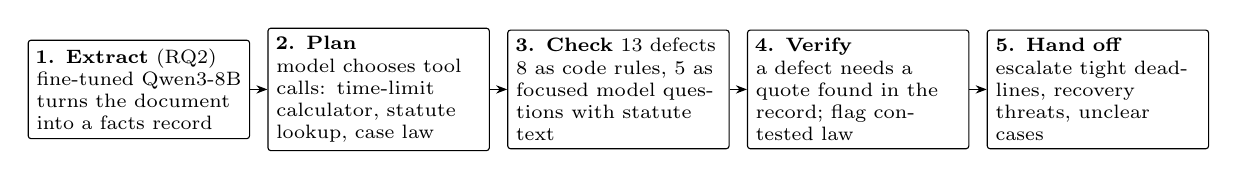
\begin{tikzpicture}[font=\scriptsize, box/.style={draw, rounded corners=1pt, text width=2.6cm, align=left, inner sep=3pt, minimum height=1.25cm}, arr/.style={-{Stealth[length=4pt]}}]
\node[box] (a) {\textbf{1. Extract} (RQ2)\\ fine-tuned Qwen3-8B turns the document into a facts record};
\node[box, right=0.22cm of a] (b) {\textbf{2. Plan}\\ model chooses tool calls: time-limit calculator, statute lookup, case law};
\node[box, right=0.22cm of b] (c) {\textbf{3. Check} 13 defects\\ 8 as code rules, 5 as focused model questions with statute text};
\node[box, right=0.22cm of c] (d) {\textbf{4. Verify}\\ a defect needs a quote found in the record; flag contested law};
\node[box, right=0.22cm of d] (e) {\textbf{5. Hand off}\\ escalate tight deadlines, recovery threats, unclear cases};
\draw[arr] (a) -- (b); \draw[arr] (b) -- (c); \draw[arr] (c) -- (d); \draw[arr] (d) -- (e);
\end{tikzpicture}
\caption{The NoticeCheck pipeline. Steps 2--5 use plain Qwen3-8B; step 1 uses our LoRA adapter. Sending a reply is the only outward action and needs human approval.}
\end{figure}

\textbf{Planning (agentic step).} The model reads the facts and decides which tools to call and with what arguments (up to 8 calls). It also lists questions for facts it is missing, such as the exact notice date.

\textbf{Tools.} \code{limitation\_check} computes the s.73/74 deadlines for a financial year, including the COVID-era extension notifications under s.168A, and reports when a result depends on an extension whose validity is disputed. \code{date\_diff} counts days between events. \code{statute\_lookup} returns the exact text of a section by number from a frozen copy of the CGST Act and Rules, split into 1,560 sections and sub-sections. \code{statute\_search} is a BM25 keyword search \cite{bm25} over the same corpus that keeps each sub-section's parent context. \code{caselaw\_search} searches 4,222 other High Court judgments (never the test cases) for points where courts disagree. \code{record\_lookup} reads a fact from the record, and \code{send\_reply} is sandboxed behind human approval.

\textbf{Checks (reasoning step).} Eight defect types follow directly from facts and tool results and are decided by short code rules: hearing, adjournment, signature, service, summary-only notice, time limit, extension validity and a single notice covering several years. If the facts a rule needs are missing, the answer is \emph{can't tell}. The other five (reply not considered, order without reasons, demand beyond the notice, s.74 used without fraud, other procedural issues) need judgement. For each, the model gets one focused question, the relevant facts and the exact statute text, and must answer with a verdict and quotes. Every finding cites its section from a fixed table that maps defect types to provisions.

\textbf{Verifier and contested law.} A \emph{defect} survives only if at least one of its quotes appears word for word in the record; otherwise it becomes \emph{can't tell}. Two points are always reported as \emph{contested} when they arise, because High Courts disagree: one notice for several financial years, and orders that are on time only because of the disputed extension notifications. These are supported with case-law search results.

\textbf{Hand-off (agentic step).} Simple rules escalate a case to a professional when the reply deadline is within 7 days, when recovery or bank attachment has started, when the case falls outside scope (for example s.74A years), when most checks are \emph{can't tell}, or when no defect was found.

\textbf{Fact extraction (fine-tuning, RQ2).} The checker needs a structured record. To produce it from a document with a small model, we fine-tuned Qwen3-8B with QLoRA (4-bit base, rank 16, two epochs, loss on the answer only) on 196 Gemini-drafted records of judgments outside every evaluation set. Training took 74 minutes on one free Kaggle T4 GPU. Untrained Qwen3-8B, the fine-tuned model and Gemini all receive the same prompt: instructions, a compact output format and the judgment text cut at 12,000 characters.

\textbf{Models and compute.} Qwen3-8B runs 4-bit through Ollama on Kaggle's free T4 GPUs with thinking turned off; Gemini 3.5 Flash Lite runs on its free API tier. One NoticeCheck case costs about 2.2 model calls, 4,500 input and 3,500 output tokens, and 3 minutes on a T4.

\textbf{An example report.} Table~\ref{tab:example} shows part of NoticeCheck's output for one test case from the Madras High Court. The court set the order aside because the officer ignored the taxpayer's reply. NoticeCheck reached the same finding with the right section and quotes, flagged the time limit as unsettled law instead of deciding it, and listed the facts it would need for the hearing check.

\begin{table}[H]
\centering\small
\begin{tabularx}{\textwidth}{l l Y}
\toprule
Check & Verdict & Evidence or missing facts \\
\midrule
Reply ignored (s.75(6)) & defect & ``the petitioner filed a reply dated 18.11.2023, providing a detailed explanation''; the order ``erroneously observed that the petitioner failed to appear for the personal hearing'' \\
Time limit (s.73(10)) & contested & order of 25.04.2024 for FY 2018-19 is on time only under the disputed extension notifications \\
Hearing, signature, service & can't tell & missing: whether a hearing date was given, whether the notice was signed, how it was served \\
Hand-off & no escalation & questions for the user: exact notice date; details of the hearing the order mentions \\
\bottomrule
\end{tabularx}
\caption{Part of NoticeCheck's report for test case HCMA011958962024 (run 2). The court's finding: the reply was not considered.}
\label{tab:example}
\end{table}

%==========================================================
\section{Experiments}

\textbf{Systems compared.}
\begin{itemize}
\item \textbf{B0}: hand-written rules for hearing, signature, service and time limit; no model.
\item \textbf{B1}: Qwen3-8B given the facts and asked for the same report in one prompt; the main baseline, since it uses the same model as NoticeCheck.
\item \textbf{B2}: Gemini 3.5 Flash Lite given the facts plus the full text of the relevant sections; a frontier reference.
\item \textbf{NoticeCheck}: the full pipeline with Qwen3-8B, run three times to measure run-to-run variation.
\item \textbf{NoticeCheck + Gemini}: the same pipeline with Gemini as the model, to separate the effect of the structure from the effect of the model.
\item \textbf{End to end}: the fine-tuned extractor reads the raw judgment and NoticeCheck checks the extracted facts, so no human-made facts are used.
\end{itemize}

\textbf{Scoring.} Only complaints the court decided are scored. A \emph{hit} is a defect call where the court found that defect; a \emph{false alarm} is a defect call where the court rejected the complaint; a \emph{miss} is anything else on a court-found defect, including \emph{can't tell} and \emph{contested}. \emph{F1} counts a hit whatever section it cites; \emph{strict F1}, the measure named in our proposal, also requires the right section. Defects flagged on points nobody argued cannot be checked against the court, so they are reported separately as \emph{unargued flags}. Differences are tested with a paired bootstrap over cases (5,000 resamples) \cite{bootstrap}. NoticeCheck was frozen before any test run; the only change after the development run fixed a verifier bug found on development cases. The repository holds the code, the answer key, every run's outputs and step-by-step traces, and a README with the commands to rebuild each number in this report.

%==========================================================
\section{Evaluation and results}

\begin{table}[H]
\centering\small\setlength{\tabcolsep}{4pt}
\begin{tabular}{l rrr r r r}
\toprule
System (125 test cases, full record) & F1 & Precision & Recall & Strict F1 & Wrong section & Unargued flags \\
\midrule
B0 rules & 0.27 & 0.81 & 0.16 & -- & -- & 1 \\
B1 Qwen3-8B, direct & 0.40 & 0.84 & 0.26 & 0.19 & 14 & 88 \\
B2 Gemini + statute & 0.50 & 0.81 & 0.37 & 0.38 & 9 & 14 \\
\textbf{NoticeCheck, 3 runs} & \textbf{0.42--0.51} & 0.76--0.83 & 0.29--0.37 & \textbf{0.42--0.51} & \textbf{0} & 29--33 \\
NoticeCheck + Gemini & 0.51 & 0.81 & 0.38 & 0.51 & 0 & 14 \\
End to end (fine-tuned extractor) & 0.38 & 0.79 & 0.25 & 0.38 & 0 & 31 \\
\bottomrule
\end{tabular}
\caption{Main results. B0 cites no sections, so it has no strict score. NoticeCheck's mean F1 over three runs is 0.47 (sd 0.04).}
\label{tab:main}
\end{table}

\textbf{RQ1.} Table~\ref{tab:main} gives the main comparison and Table~\ref{tab:rq1} the three tests fixed in the proposal. The main test is met by a wide margin in every run. Most of that margin comes from citing the law correctly: B1 cites a wrong section on 14 of its 27 hits, for example s.75(4) or s.73(9) for an ignored reply where the rule is s.75(6), while NoticeCheck never does. On detection alone (any section) the gain over B1 is +0.03, +0.11 and +0.07, and no interval excludes zero. The false-alarm test fails: NoticeCheck makes 8--11 false alarms against B1's 5, most of them on service, where it treats a notice uploaded only to the portal's ``Additional Notices'' tab as improperly served and the court in those cases disagreed. NoticeCheck is also far more restrained than B1, with about 30 unargued flags instead of 88 (difference about $-57$, 95\% interval roughly $[-82, -35]$).

\begin{table}[H]
\centering\small
\begin{tabularx}{\textwidth}{Y Y l}
\toprule
Test from the proposal & Result & Met \\
\midrule
Strict F1 at least 10 points above B1, interval above zero & +0.23 [0.11, 0.35]; +0.32 [0.18, 0.44]; +0.28 [0.14, 0.40] & Yes \\
False-alarm rate not above B1's (0.14) & 0.22, 0.22, 0.30 & No \\
Beat the rule checklist on reasoning-dependent defects & B0 finds none; NoticeCheck 0.34--0.52 & Yes \\
\bottomrule
\end{tabularx}
\caption{RQ1 against the falsification criteria (three NoticeCheck runs; brackets are 95\% intervals).}
\label{tab:rq1}
\end{table}

\textbf{Against the frontier model.} On detection, NoticeCheck and B2 are level ($-0.08$, $0.00$, $-0.04$; all intervals include zero). With the right section required NoticeCheck is ahead (+0.04, +0.12, +0.08). Putting Gemini inside our pipeline gives the same detection F1 as B2 (0.51 vs 0.50) but a strict F1 13 points higher (interval above zero). With either model the pipeline reaches about 0.50, which suggests the limit lies in what the records contain rather than in the model.

\textbf{Why recall is low.} Of the 104 defects courts found, NoticeCheck (run 2) called 38 defects, answered \emph{can't tell} on 49, \emph{contested} on 10 and \emph{no defect} on 7. Hearing defects explain 29 of the 49 \emph{can't tell} answers: judgments state the conclusion (``the order was passed without affording an opportunity of hearing'') but rarely the dates behind it, and copying the court's conclusion into the facts would leak the answer. The \emph{no defect} answers arise in cases like one from the fresh set (Section~\ref{sec:fresh}): the court held that no hearing was offered, but the record held only the petitioner's account that a hearing notice was issued, so NoticeCheck answered \emph{no defect}. All 10 \emph{contested} misses are notices covering several years, which the system deliberately refers to a lawyer because High Courts disagree; it flagged 81\% of the 26 contested points in the test set. Precision, in contrast, is high for every system (0.76--0.84).

\textbf{Run-to-run variation and other views.} The three runs differ significantly (run 2 minus run 1 is +0.08) even at temperature 0, because Ollama batches requests on the GPU; they agree on 89\% of verdicts. With the notice alone, most defects have not happened yet, and NoticeCheck (0.29), B2 (0.30) and B0 (0.27) score alike. On the held-out Karnataka court, every system working from checked facts finds 0 of 6 defects: the judgments are short and state no hearing or notice details.

\textbf{Capabilities in numbers.} NoticeCheck made about 630 tool calls per run with valid arguments 95--97\% of the time (Gemini 100\%); almost every error was a malformed financial year, and the model recovered in 15 of 50 such cases. It used the time-limit calculator in 90--98\% of cases where the dates allowed it, and made no unsafe action. The verifier turned 4--7 defect calls per run into \emph{can't tell}; only one of these, across three runs, was a defect the court had found. Keyword search over the statute is weak (right section in the top five for 11\% of complaint texts, 8\% without the hierarchy), so the design fetches law text by section number. The hand-off rules caught 73\% of cases needing escalation at 41\% precision (measured on the one hand-off reason the answer key covers).

\textbf{RQ2: fact extraction.} Table~\ref{tab:rq2} compares the extractors field by field against our checked facts (notice date, reply due, hearing given, service mode, order date, section, financial years and others). Fine-tuning adds 28 points of field F1 (interval [0.22, 0.34]) and lifts the held-out court from 0.50 to 0.89. The untrained model fills in values the judgment never states, so most of what it reports is wrong. The fine-tuned model sometimes repeats a quote until it hits the 2,048-token limit; keeping the valid part of such outputs raises its F1 to 0.88. The Gemini drafts score higher, but that number is inflated because our reviewers corrected those very drafts to build the answer key. The fine-tuned model therefore comes close to the large model without matching it.

\begin{table}[H]
\centering\small
\begin{tabular}{l rrr rr}
\toprule
Extractor (125 test judgments) & Field F1 & Precision & Recall & Events F1 & Schema-valid \\
\midrule
Qwen3-8B, untrained & 0.52 & 0.38 & 0.82 & 0.42 & 31/125 \\
\textbf{Qwen3-8B + our LoRA} & \textbf{0.80} & \textbf{0.90} & 0.72 & 0.71 & 103/125 \\
\quad cut-off outputs repaired & 0.88 & 0.91 & 0.84 & 0.72 & -- \\
Gemini drafts (inflated, see text) & 0.95 & 0.96 & 0.94 & 0.96 & 125/125 \\
\bottomrule
\end{tabular}
\caption{RQ2: extracting the facts of a proceeding from the judgment text.}
\label{tab:rq2}
\end{table}

\textbf{End to end.} With the fine-tuned extractor feeding NoticeCheck, the whole system works from the judgment alone at F1 0.38, with the same precision (0.79) and restraint (31 unargued flags) as on checked facts, and it still beats B1 on strict F1 by 19 points (interval above zero) although B1 received checked facts. The untrained extractor gives a higher F1 (0.56) for the wrong reason: it invented ``hearing date given'' in 77 of 125 cases where the judgment is silent, so NoticeCheck flagged defects almost everywhere (158 defect calls, 97 unargued), and 39\% of its evidence quotes do not appear in the judgment. Because courts upheld most argued complaints, blanket flagging often lands. Defect F1 alone can reward a hallucinating extractor; field accuracy, unargued flags and quote checks expose it.

\textbf{Fresh cases checked by hand.}\label{sec:fresh} Twenty judgments picked after the freeze, never used before, went through the full end-to-end system, and the four of us checked its 81 calls against the judgments. All 8 defect calls judged correct were defects the court found, and all 6 defect calls on points nobody argued were judged wrong, which confirms that unargued flags are mostly false alarms. ``No defect'' was right in 94\% of the calls a reader could verify, and ``contested'' fitted the case in 71\%. About 14 court-found defects were missed, mostly ``no hearing'' in one recurring Madras order format, giving an estimated recall of 0.36--0.40, in line with the end-to-end test result.

\textbf{Synthetic stress set.} Real judgments leave many facts out and contain no case known to be fully valid, so they cannot show how a system behaves when every fact is stated, or how often it raises false alarms on a proceeding with nothing wrong. We therefore generated 100 records from the DRC-01 template: 8 for each of seven defect types (no hearing, unsigned notice or order, summary-only notice, notice not served, time limit missed, reply ignored, order without reasons) and 44 clean records. Each record states every fact the seven checks need, giving 56 planted defects and 644 clean checks.

\begin{table}[H]
\centering\small
\begin{tabular}{l rrr r r}
\toprule
System (100 synthetic records) & F1 & Precision & Recall & Strict F1 & False alarms (of 644) \\
\midrule
B0 rules & 0.40 & 1.00 & 0.25 & -- & 0 \\
B1 Qwen3-8B, direct & 0.74 & 0.74 & 0.75 & 0.25 & 15 \\
B2 Gemini + statute & 0.91 & 1.00 & 0.84 & 0.58 & 0 \\
\textbf{NoticeCheck (Qwen3-8B)} & \textbf{0.91} & 0.88 & \textbf{0.95} & \textbf{0.91} & 7 \\
NoticeCheck + Gemini & 0.99 & 0.98 & 1.00 & 0.99 & 1 \\
\bottomrule
\end{tabular}
\caption{Synthetic records with planted defects and clean controls.}
\label{tab:synthetic}
\end{table}

With every fact stated, NoticeCheck beats the same model used directly even on detection: +0.17 F1 (interval [0.08, 0.27]), which the real test set could not show because its records lack the facts. With the right section required the gap grows to +0.67, since B1 cites a wrong section on 28 of its 42 hits. Time limits show the value of the calculator most clearly: B1 caught 2 of the 8 late orders and raised 11 false time-limit alarms on clean records, and B2, which has the statute text but no calculator, missed all 8; NoticeCheck caught all 8 with no false alarm, with either model. On the 644 clean checks NoticeCheck raised 7 false alarms against B1's 15 (the interval just includes zero), so on valid proceedings it is the more cautious of the two, and all three RQ1 tests from the proposal are met on this set. Six of its seven false alarms called an order ``without reasons'' in records whose planted defect was the ignored reply. Its rule-based checks were perfect, which is partly by construction since the rules are code over facts that are all present; on the two model-judged types Qwen scored 0.81 (B1 0.83) and Gemini 0.98, so these judgement calls depend on the strength of the model rather than on the structure.

%==========================================================
\section{Ablations}

Each ablation removes one component in code and was run once on the test set.

\begin{table}[H]
\centering\small
\begin{tabular}{l rrr rr}
\toprule
Version & F1 & Precision & Recall & False alarms & Unargued flags \\
\midrule
Full NoticeCheck (3 runs) & 0.42--0.51 & 0.76--0.83 & 0.29--0.37 & 8--11 & 29--33 \\
No tools (model judges dates itself) & 0.48 & 0.83 & 0.34 & 7 & 48 \\
No retrieval (no statute text for the model) & 0.49 & 0.84 & 0.35 & 7 & 30 \\
No verifier (findings not checked) & 0.45 & 0.77 & 0.32 & 10 & 30 \\
No hand-off (never escalates) & 0.46 & 0.82 & 0.32 & 7 & 32 \\
\bottomrule
\end{tabular}
\caption{Ablations on the 125 test cases.}
\end{table}

Every ablation falls inside the full system's run-to-run range, so on 125 cases no single component can be shown to raise F1. Two effects are visible: without tools the unargued flags rise from about 30 to 48, and without the verifier false alarms are highest. Removing the statute text changes little because the model already knows the main sections and the citation itself comes from the provision table. With 125 cases, effects of this size cannot be measured reliably.

%==========================================================
\section{Limitations}
\begin{itemize}
\item \textbf{No real notices.} Every input is a proceeding as described in a High Court judgment, not the notice itself.
\item \textbf{Missing facts.} Judgments often give conclusions without dates, which caps recall for every system; \emph{can't tell} is frequently the correct answer.
\item \textbf{Model-drafted labels.} Gemini drafted the records before human correction, which may favour the Gemini baseline and inflates its extraction score.
\item \textbf{Small test set.} With 104 court-found defects, differences below about 8--10 F1 points cannot be confirmed, and the ablations cannot separate components.
\item \textbf{Variation and coverage.} The local model varies between runs even at temperature 0; Madras and Delhi dominate the data; the held-out court has only 6 defects; the fresh check covers 20 cases and its reviewers saw the system's answers; the synthetic records are template-built and cleaner than real ones.
\end{itemize}

\textbf{Responsible use.} NoticeCheck is a screening aid, not legal advice. It never judges whether tax is owed, it attaches the law and the evidence to every point so a reader can check it, and it refers unsettled questions, urgent deadlines and cases where it finds nothing to a professional. Its only outward action, sending a reply, is sandboxed behind explicit human approval. All judgments used are public court records released under CC-BY-4.0.

%==========================================================
\section{Conclusion}
NoticeCheck shows that a free 8B model, placed inside a fixed structure of planning, tools, statute lookup, verification and hand-off, can check the procedure of GST tax demands with high precision, cite the correct law every time, and raise far fewer flags on points nobody argued than the bare model. On the measure set in our proposal it beats that baseline by 23--32 F1 points, though it raises slightly more false alarms and its detection gain alone is not significant. It matches a commercial model at finding defects and cites the law more accurately. When every fact is stated, as in our synthetic records, it finds 95\% of planted defects, beats the bare model on detection as well, raises half as many false alarms on valid proceedings, and catches late orders that a frontier model without a calculator misses. A LoRA-tuned copy of the same model extracts the facts well enough for the whole system to run from a judgment alone. The main limit is the data: judgments often omit the facts a check needs. Testing on real notices, together with the taxpayer's own documents, is the most useful next step.

%==========================================================
\small
\begin{thebibliography}{99}\setlength{\itemsep}{1pt}
\bibitem{lexglue} I.~Chalkidis, A.~Jana, D.~Hartung, M.~Bommarito, I.~Androutsopoulos, D.~M.~Katz, N.~Aletras. LexGLUE: A benchmark dataset for legal language understanding in English. \emph{ACL}, 2022.
\bibitem{legalbench} N.~Guha et al. LegalBench: A collaboratively built benchmark for measuring legal reasoning in large language models. \emph{NeurIPS Datasets and Benchmarks}, 2023.
\bibitem{sara} N.~Holzenberger, A.~Blair-Stanek, B.~Van~Durme. A dataset for statutory reasoning in tax law entailment and question answering. \emph{Natural Legal Language Processing Workshop}, 2020.
\bibitem{blairstanek} A.~Blair-Stanek, N.~Holzenberger, B.~Van~Durme. Can GPT-3 perform statutory reasoning? \emph{ICAIL}, 2023.
\bibitem{nay} J.~J.~Nay et al. Large language models as tax attorneys: a case study in legal capabilities emergence. \emph{Philosophical Transactions of the Royal Society A}, 2024.
\bibitem{dahl} M.~Dahl, V.~Magesh, M.~Suzgun, D.~E.~Ho. Large legal fictions: Profiling legal hallucinations in large language models. \emph{Journal of Legal Analysis}, 2024.
\bibitem{magesh} V.~Magesh, F.~Surani, M.~Dahl, M.~Suzgun, C.~D.~Manning, D.~E.~Ho. Hallucination-free? Assessing the reliability of leading AI legal research tools. arXiv:2405.20362, 2024.
\bibitem{ildc} V.~Malik et al. ILDC for CJPE: Indian legal documents corpus for court judgment prediction and explanation. \emph{ACL}, 2021.
\bibitem{rhetorical} P.~Kalamkar et al. Corpus for automatic structuring of legal documents. \emph{LREC}, 2022.
\bibitem{rag} P.~Lewis et al. Retrieval-augmented generation for knowledge-intensive NLP tasks. \emph{NeurIPS}, 2020.
\bibitem{alce} T.~Gao, H.~Yen, J.~Yu, D.~Chen. Enabling large language models to generate text with citations. \emph{EMNLP}, 2023.
\bibitem{toolformer} T.~Schick et al. Toolformer: Language models can teach themselves to use tools. \emph{NeurIPS}, 2023.
\bibitem{react} S.~Yao et al. ReAct: Synergizing reasoning and acting in language models. \emph{ICLR}, 2023.
\bibitem{cot} J.~Wei et al. Chain-of-thought prompting elicits reasoning in large language models. \emph{NeurIPS}, 2022.
\bibitem{intragent} IntrAgent. arXiv:2604.22861, 2026. % TODO: add authors and full title
\bibitem{lora} E.~J.~Hu et al. LoRA: Low-rank adaptation of large language models. \emph{ICLR}, 2022.
\bibitem{qlora} T.~Dettmers, A.~Pagnoni, A.~Holtzman, L.~Zettlemoyer. QLoRA: Efficient finetuning of quantized LLMs. \emph{NeurIPS}, 2023.
\bibitem{qwen3} Qwen Team. Qwen3 technical report. arXiv:2505.09388, 2025.
\bibitem{bm25} S.~Robertson, H.~Zaragoza. The probabilistic relevance framework: BM25 and beyond. \emph{Foundations and Trends in Information Retrieval}, 3(4), 2009.
\bibitem{cohen} J.~Cohen. A coefficient of agreement for nominal scales. \emph{Educational and Psychological Measurement}, 20(1), 1960.
\bibitem{bootstrap} B.~Efron, R.~J.~Tibshirani. \emph{An Introduction to the Bootstrap}. Chapman \& Hall, 1993.
\bibitem{awsdata} Indian High Court Judgments, AWS Open Data Registry (\url{https://registry.opendata.aws/indian-high-court-judgments/}), CC-BY-4.0. Accessed October 2026.
\bibitem{cgst} The Central Goods and Services Tax Act, 2017, and CGST Rules, 2017. India Code and CBIC, versions as of 2026.
\end{thebibliography}

\end{document}
